\subsection{Περιγραφή Πειράματος}

Το πείραμα διεξήχθη σε εσωτερικό κλειστό χώρο, σε αίθουσα του εργαστηρίου (\hyperref[fig:experimentLab]{\schema~\ref*{fig:experimentLab}}). Κάθε εθέλοντης προσέρχοταν στο εργαστήριο και, προτού εισέλθει στην αίθουσα, λάμβανε ορισμένες σύντομες οδηγίες. Ειδικότερα, ενημερώναμε τους χρήστες για τα σκέλη του πειράματος και τον τρόπο διεξαγωγής τους. Επιπλέον, εξηγούσαμε τον τρόπο χρήσης της εφαρμογής, δηλαδή τις διαθέσιμες φωνητικές εντολές, καθώς τα διάφορα είδη ειδοποιήσεων, τα οποία θα λάμβαναν, αλλά τονίσαμε, επίσης, ορισμένα σφάλματα και λανθασμένες συμπεριφόρες της εφαρμογής, τις οποίες εντοπίσαμε κατά τις δοκιμές μας και γνωρίζαμε ότι θα συναντούσαν οι χρήστες, και τον τρόπο αντιμετώπισής τους. Στη συνέχεια, αφού καλύπταμε τα μάτια του εθελοντή με ένα πανί, εισέρχοταν στο χώρο διεξαγωγής του πειράματος. Με αυτό τον τρόπο εξασφλίζαμε ότι ο χρήστης δε γνωρίζει τη διάταξη του χώρου, καθώς και το πλήθος των εμποδίων, το είδος αυτών και τη θέση τους.

\begin{figure}[!h]
  \centering
  \begin{subfigure}{0.25\textwidth}
    \centering
    \includegraphics[width=0.9\linewidth]{images/experimentSector1.jpg}
    \caption{Τμήμα 1}\label{fig:experimentSector1}
  \end{subfigure}%
  \begin{subfigure}{0.25\textwidth}
    \centering
    \includegraphics[width=0.9\linewidth]{images/experimentSector2.jpg}
    \caption{Τμήμα 2}\label{fig:experimentSector2}
  \end{subfigure}%
  \begin{subfigure}{0.25\textwidth}
    \centering
    \includegraphics[width=0.9\linewidth]{images/experimentSector3.jpg}
    \caption{Τμήμα 3}\label{fig:experimentSector3}
  \end{subfigure}%
  \begin{subfigure}{0.25\textwidth}
    \centering
    \includegraphics[width=0.9\linewidth]{images/experimentSector4.jpg}
    \caption{Τμήμα 4}\label{fig:experimentSector4}
  \end{subfigure}%
  \caption{Χώρος διεξαγωγής του πειράματος}\label{fig:experimentLab}
\end{figure}

Το πείραμα χωρίζεται σε δύο σκέλη, όπου, και στα δύο, ο εθελοντής καλείται να περιηγηθεί στην αίθουσα με όσο τον δυνατό μεγαλύτερη ασφάλεια (δηλαδή χωρίς να <<συγκρουστεί>> με κάποιο εμπόδιο) μέχρι να φθάσει στο τέλος της διαδρομής, το οποίο, λόγω της διάταξης του χώρου, ταυτίζεται με το σημείο έναρξης. Κατά το πρώτο σκέλος, ο χρήστης περιηγούταν στο χώρο χρησιμοποιώντας ένα μπαστούνι τυφλών (\hyperref[fig:experimentCane]{\schema~\ref*{fig:experimentCane}}), η οποία αποτελεί και τη πιο συνηθισμένη λύση για άτομα με απώλεια όρασης. Αφού ολοκληρώσει τη διαδρομή, επαναλαμβάνει το πείραμα, αυτή τη φορά χρησιμοποιώντας την συσκευή HoloLens 2 και την εφαρμογή που αναπτύξαμε για αυτήν (\hyperref[fig:experimentHololens]{\schema~\ref*{fig:experimentHololens}}). Μετά το πέρας και του δεύτερου σκέλους, ο εθελοντής συμπληρώνει ένα ερωτηματολογίο, απαντά, προφορικά ή γραπτώς, σε μερικές ερωτήσεις ανοικτού τύπου και η διαδικασία ολοκληρώνεται.
% Αναλυτική περιγραφή των πειραμάτων που θα διεξαχθούν\\
% Ανάλυση περιορισμών > Ως προς το χώρο, τους συμμετέχοντες κλπ

\begin{figure}[!h]
  \centering
  \begin{subfigure}{0.5\textwidth}
    \centering
    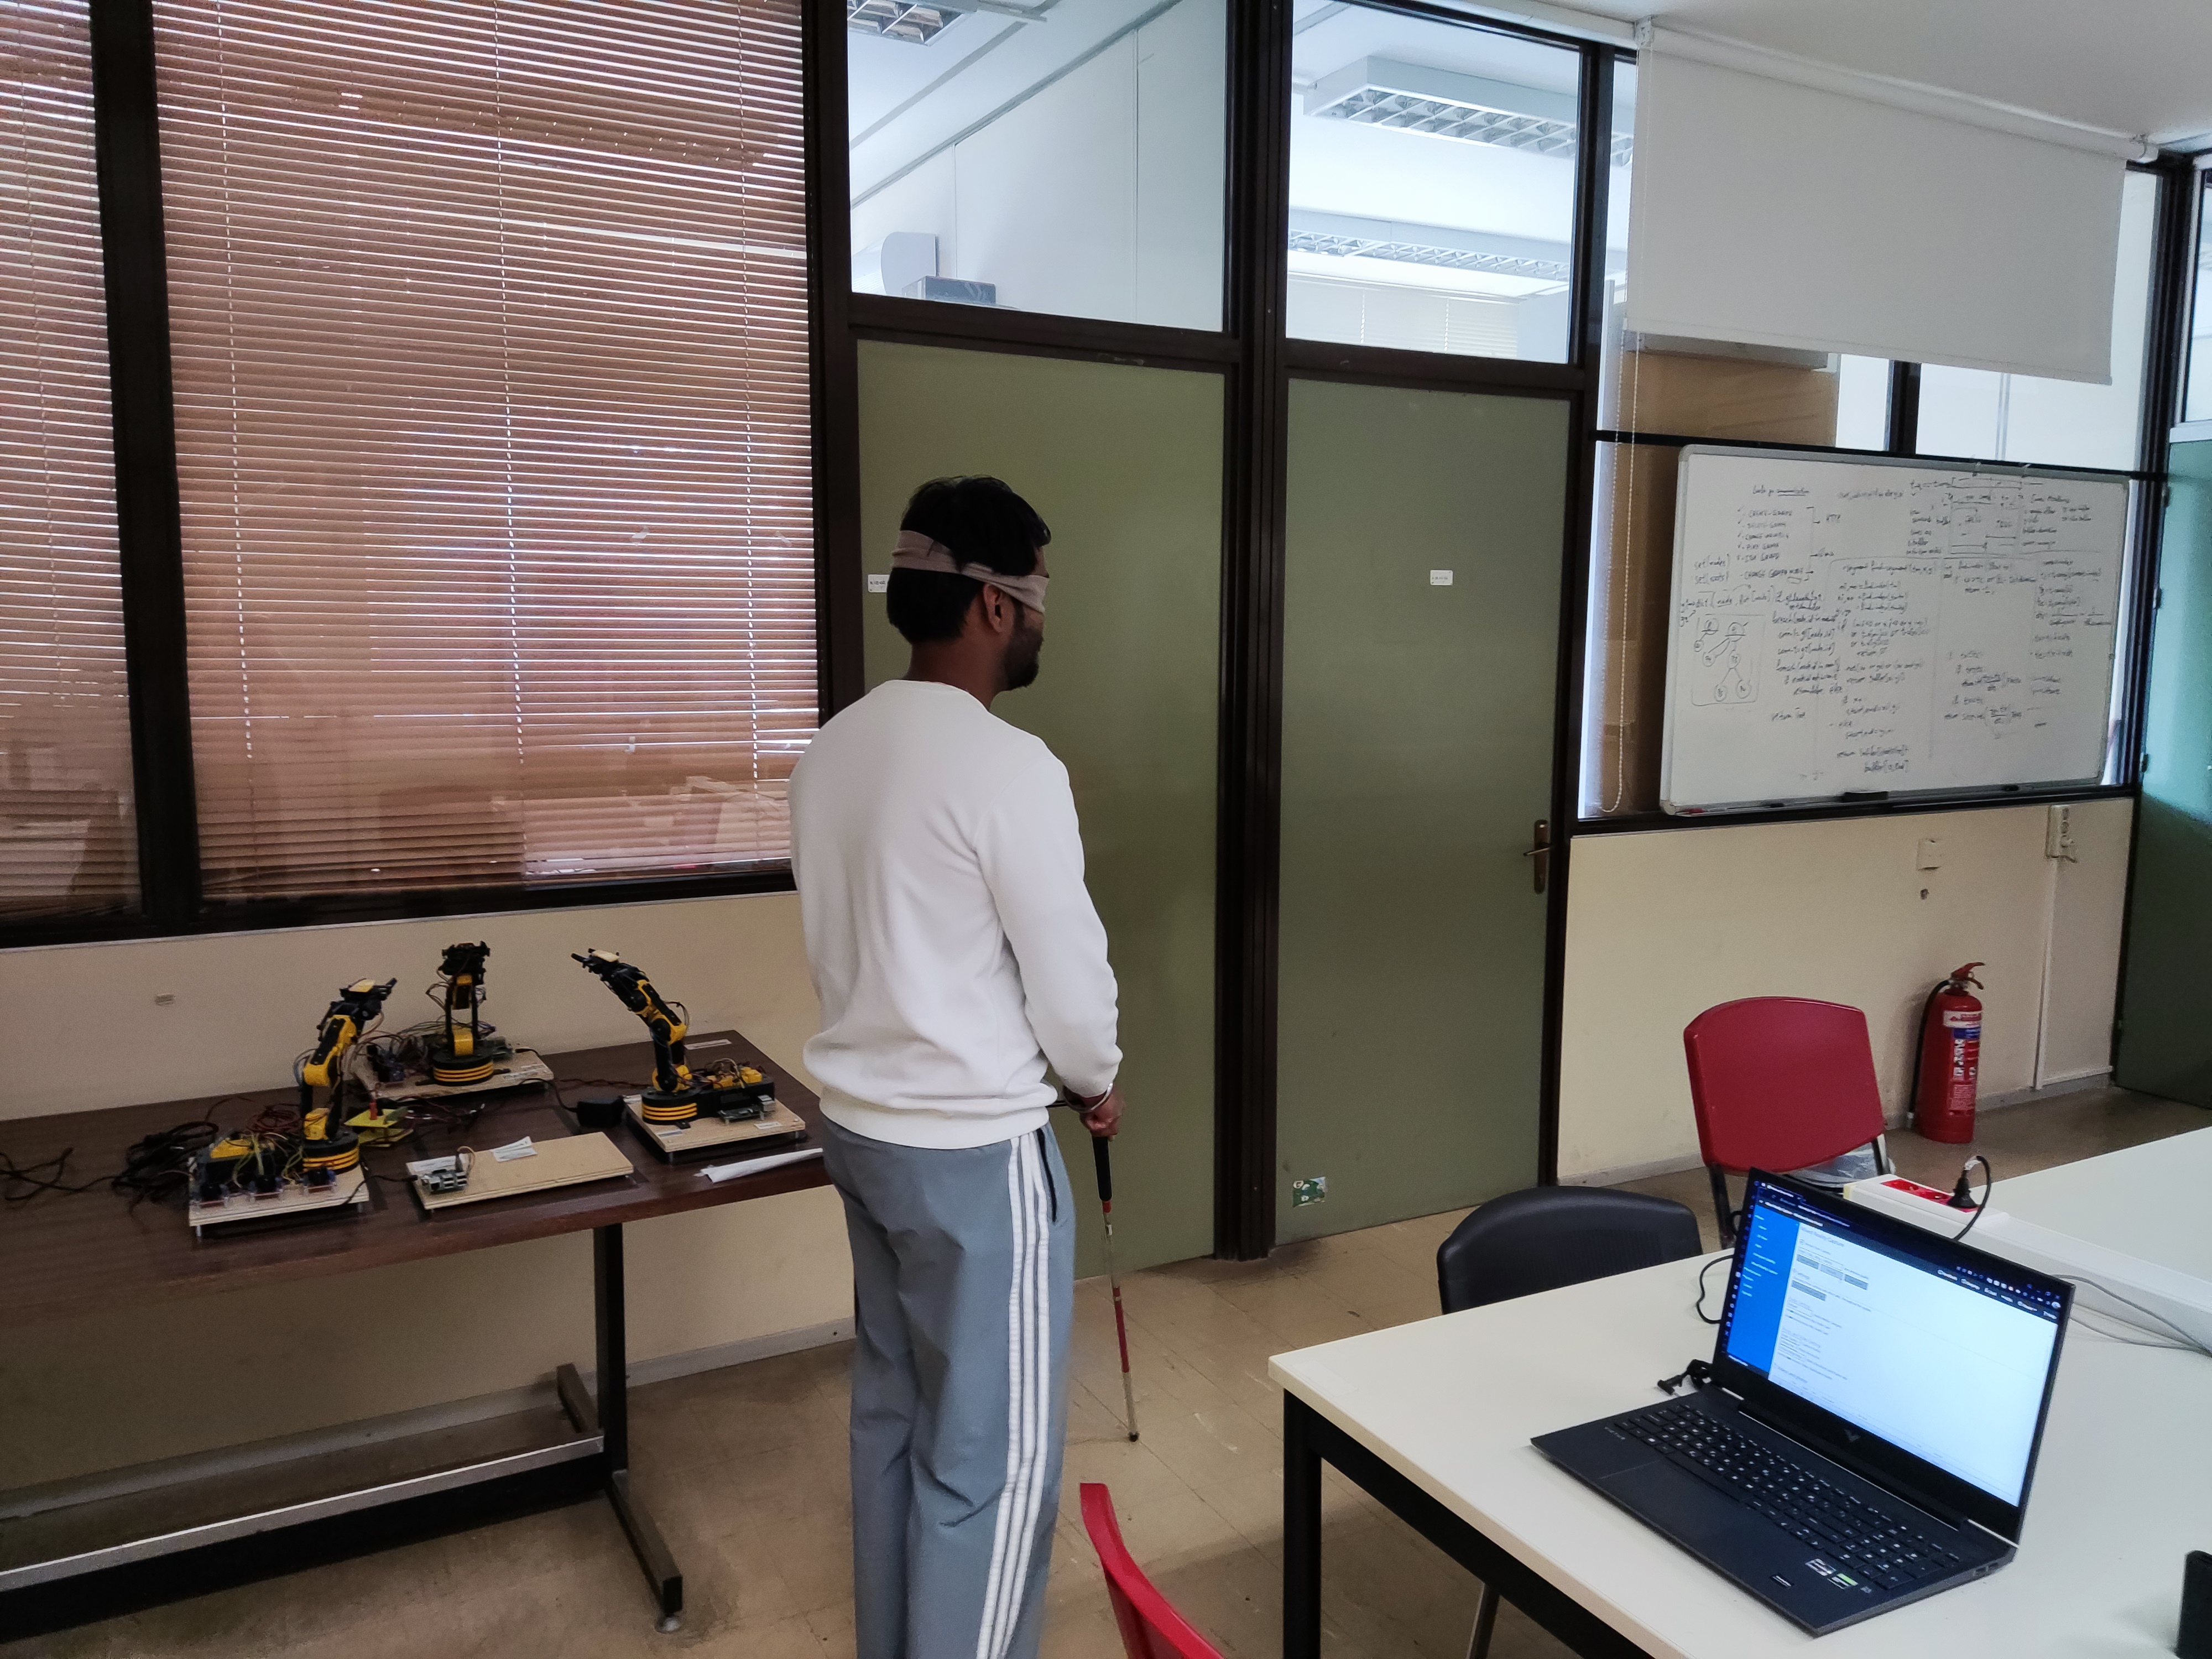
\includegraphics[width=0.7\linewidth]{images/experimentCane.jpg}
    \caption{Χρήση του μπαστουνιού}\label{fig:experimentCane}
  \end{subfigure}%
  \begin{subfigure}{0.5\textwidth}
    \centering
    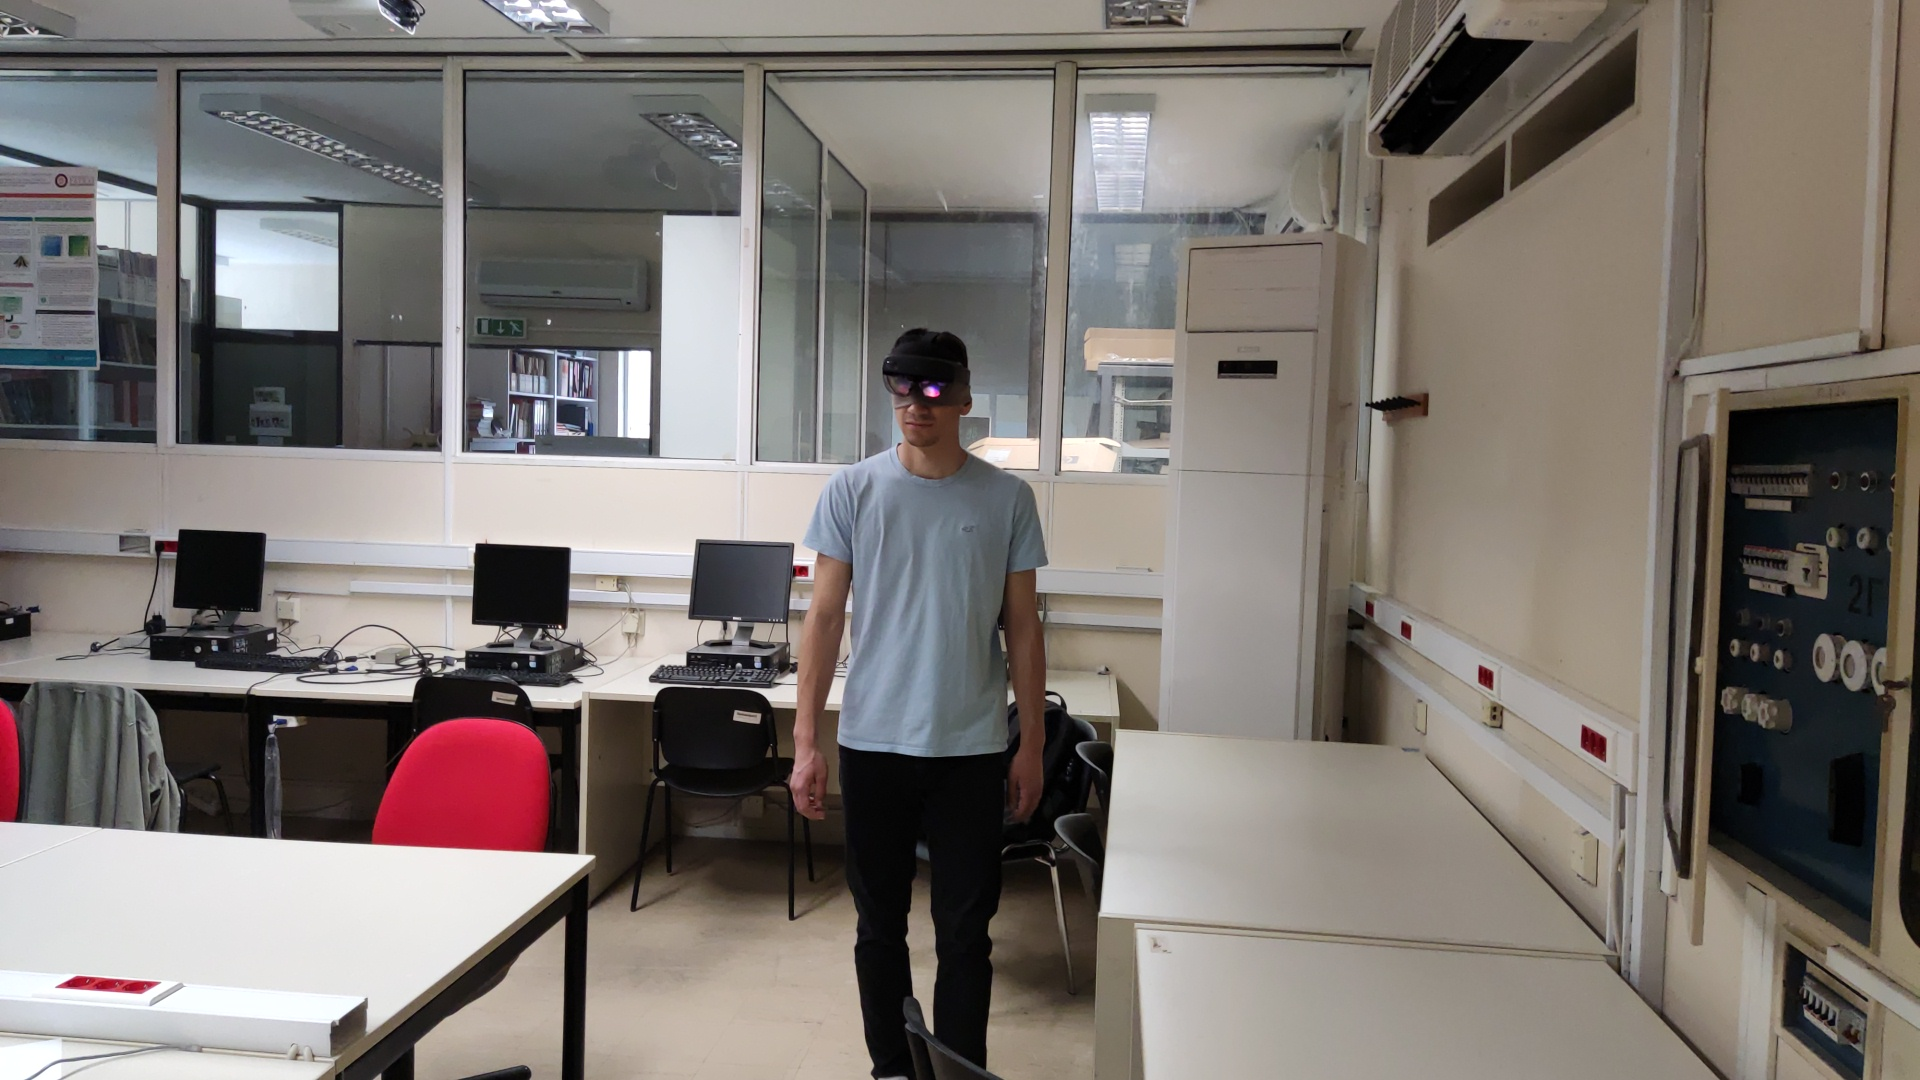
\includegraphics[width=0.9\linewidth]{images/experimentHololens.jpg}
    \caption{Χρήση εφαρμογής στο HoloLens 2}\label{fig:experimentHololens}
  \end{subfigure}%
  \caption{Εθελοντές χρησιμοποιούν τους δύο διαφορετικούς τρόπους περιήγησης στο χώρο}\label{fig:experimentNavMethods}
\end{figure}

\subsection{Προδιαγραφές Αξιολόγησης}\label{subsec:experimentSpecsForEvaluation}
Το πείραμα έλαβε χώρο στην κύρια αίθουσα του εργαστηρίου Συστημάτων Υπολογιστών. Επιλέχθηκε ένας εσωτερικός κλειστός χώρος, λόγω των περιορισμών που θέτει το ίδιο το HoloLens 2 για την ορθή χαρτογράφηση του χώρου, η οποία εξαρτάται από τον φωτισμό και τις επιφάνειές του~\cite{mattzmsft_2023_spatial}. Επιπλέον, υπήρχε μεγαλύτερος έλεγχος στις συνθήκες διεξαγωγής του πειράματος, καθώς μπορούσαμε να επιλέξουμε τα εμπόδια και τη θέση τους στο χώρο, ενώ το ρίσκο για κάποιο αναπάντεχο γεγονός κατά την διεξαγωγή ήταν πολύ μικρότερο σε αντίθεση με το αν γινόταν σε έναν ανοιχτό, εξωτερικό χώρο.
Πριν εισέλθουν οι εθελοντές στο χώρο, παρείχαμε οδηγίες για τον τρόπο χρήσης της εφαρμογής, ενώ υπήρξε και ιδιαίτερη μνεία σε δύο άλυτα προβλήματα της εφαρμογής:
\begin{itemize}
    \item Μίξη των προειδοποιητικών ήχων: κατά τη χρήση της εφαρμογής, λόγω της κίνησης του κεφαλιού του χρήστη όσο αυτός περπατά, οπότε και του headset, η εφαρμογή μπορεί να εντοπίσει κάποιο διαφορετικό σημείο του mesh ως πλησιέστερο προς το χρήστη. Ως αποτέλεσμα, κατά την κίνηση του χρήστη, είναι πιθανό να αναπαράγονται πολλοί, διαφορετικοί προειδοποιητικοί ήχοι σε πολύ σύντομο χρονικό διάστημα. Προτάθηκε στους χρήστες, αν αυτό συμβεί, να παραμείνουν σταθεροί στο σημείο εως ότου η συσκευή εντοπίσει το σωστό πλησιέστερο σημείο του mesh και να αναπαράξει το σωστό προειδοποιητικό ήχο.
    \item Δημιουργία `hallucinations': είναι πιθανό, σε δυναμικά περιβάλλοντα, όπου άτομα ή αντικείμενα μετακινούνται, να δημιουργηθούν `hallucinations', δηλαδή 3D αναπαραστάσεις αντικειμένων να τοποθετηθούν σε σημείο, στο οποίο δε βρίσκεται πλέον το αντικείμενο~\cite{mattzmsft_2023_spatial}. Προσπαθήσαμε να επιλύσουμε το θέμα αυτό, θέτοντας την τιμή για το Update Interval της χωρικής χαρτογράφησης στη μικρότερη δυνατή τιμή~\cite{davidklinems_2022_configuring}. Ωστόσο, και σε αυτή την περίπτωση, απαιτούνται περίπου 3-4 δευτερόλεπτα, ώστε να αντικατροπτιστεί μια αλλαγή του περιβάλλοντος στο mesh. Για το λόγο αυτό, πριν ο εθελοντής χρησιμοποιήσει την εφαρμογή, πραγματοποιούμε μια αρχική χαρτογράφηση του χώρου, ώστε να αφαιρέσουμε πιθανά hallucinations, που έχουν παραμείνει. %chktex-file 8
\end{itemize}

Στο πείραμα συμμετείχαν δέκα άτομα (πέντε άντρες και πέντε γυναίκες), ηλικιών από 21 έως 47 ετών και με μέση ηλικία τα 25.7 έτη. Από τα άτομα αυτά, τέσσερις είχαν κάποια προηγούμενη εμπειρία με τεχνολογία εκτεταμένης πραγματικότητας και, ειδικότερα, ένας είχε εμπειρία με την επαυξημένη πραγματικότητα (AR), ένας με την εικονική (VR) και δύο και με τα δύο είδη πραγματικότητας. Η πλειονότητα των εθελοντών ένιωθε ότι έχει ελάχιστη εξοικείωση με την τεχνολογία AR (\hyperref[fig:questARFamiliariaty]{\schema~\ref*{fig:questARFamiliariaty}}).

\begin{figure}[!h]
    \centering
    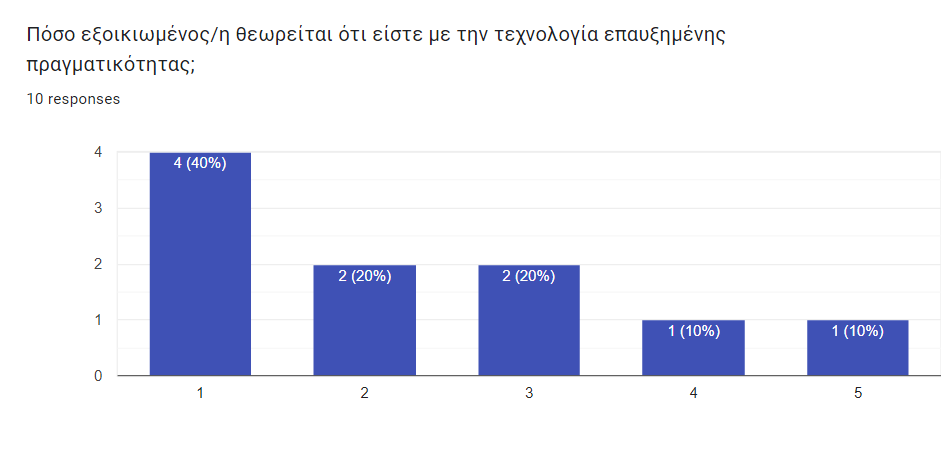
\includegraphics[width=1\textwidth]{images/questionnaire_familiarityAR.png}
    \caption{Απαντήσεις για το επίπεδο εξοικείωσης των εθελοντών με την επαυξημένη πραγματικότητα}\label{fig:questARFamiliariaty}
\end{figure}

Τέλος, έξι στους δέκα ανέφεραν ότι ήταν προηγουμένως εξοικειωμένοι με τη διάταξη του χώρου. Ωστόσο, καλύπτοντας τα μάτια των εθελοντών πριν εισέλθουν στο χώρο, εξασφαλίζαμε ότι κανένας εθελοντής δε γνώριζε τη θέση των εμποδίων σε αυτόν.

Για την εκτέλεση του πειράματος, αποφασίσαμε όλοι οι εθελοντές να πραγματοποιήσουν και τα δύο σκέλη/tasks αυτού, δηλαδή πραγματοποιήσαμε ένα πείραμα within-subjects~\cite{bhandari_2021_withinsubjects}. Επιλέξαμε αυτό το τύπο πειράματος, λόγω του μικρού αριθμού εθελοντών που διαθέταμε και της πολυπλοκότητας των tasks~\cite{lazar_2017_research}. Για να μειώσουμε το learning effect, όπου οι εθελοντές μαθαίνουν και είναι περισσότερο προετοιμασμένοι μετά την ολοκλήρωση του πρώτου task, αναθέσαμε στους μισούς εθελοντές να χρησιμοποιήσουν πρώτα το μπαστούνι τυφλών (πρώτο σκέλος) και έπειτα την εφαρμογή (δεύτερο σκέλος), ενώ οι υπόλοιποι εθελοντές πραγματοποίησαν τα σκέλη με την αντίστροφη σειρά.

Κατά την εκτέλεση και των δύο σκελών, καταγράφαμε το χρόνο που απαιτείται για να ολοκληρωθεί κάθε task, συνολικά και ανά τμήμα, καθώς είχαμε χωρίσει την περιήγηση σε τέσσερα τμήματα. Επίσης, σημειώναμε το πλήθος σφαλμάτων που έκαναν οι εθελοντές κατά την πραγματοποίηση ενός task. Ως σφάλμα σημειώσαμε κάθε σύγκρουση ενός εθελοντή με ένα εμπόδιο, καθώς και όταν κατευθυνόταν προς τη λάθος κατεύθυνση και όχι προς το τέλος της διαδρομής.

Τέλος, για την αξιολόγηση της εφαρμογής και της χρηστικότητάς της, χρησιμοποιήθηκε το ερωτηματολογίο System Usability Scale (SUS), το οποίο περιέχει δέκα προτάσεις~\cite{brooke_1995_sus}. Σε κάθε πρόταση, ο χρήστης επιλέγει έναν ακέραιο αριθμό από την κλίμακα 1 έως 5, ανάλογα με το πόσο συμφωνεί με όσα αναφέρει η πρόταση. Ο αριθμός 1 στην κλίμακα αντιστοιχεί στην απάντηση `Διαφωνώ Απόλυτα', ενώ το 5 στην απάντηση `Συμφωνώ Απόλυτα'. Για να προκύψει η τελική βαθμολογία, η οποία είναι ένας αριθμός μεταξύ του 0 και του 100, εφαρμόζουμε τον ακόλουθο μαθηματικό τύπο, όπου $n$ είναι ο αριθμός της ερώτησης και $x_n$ η τιμή της κλίμακας που επέλεξε ο χρήστης για την ερώτηση $n$:

\[
  \text{SUS Score} = 2.5 \times ( \sum_{n=1}^{5}(x_{2n - 1} - 1) + \sum_{n=1}^{5}(5 - x_{2n}))
\]

Στο τέλος του ερωτηματολογίου, προσθέσαμε τρεις ερωτήσεις ανοικτού τύπου, έτσι ώστε να καταγράψουμε καλύτερα την εμπειρία των εθελοντών με την εφαρμογή, δυσκολίες που αντιμετώπισαν, καθώς και τις προτάσεις τους για τη βελτίωσή της. Το ερωτηματολόγιο SUS και οι ανοικτού τύπου ερωτήσεις παρατίθενται στο \hyperref[ch:appendixB]{Παράρτημα Β}.

% \subsection{Διεξαγωγή Πειράματος}
% Χώρος διεξαγωγής